\documentclass[12pt,a4paper,twoside]{report}

\usepackage[utf8]{inputenc}
\usepackage{graphicx}
\graphicspath{ {./../figures/} }
\usepackage{caption}
\usepackage{subcaption}
\usepackage{xcolor}
\usepackage{hyperref}
\usepackage{imakeidx} % for index
\makeindex[columns=3, title=Alphabetical Index]
\usepackage{soul} % allow wrapping of underlined text, via \ul{...}
\usepackage{natbib} % for bibliography
\usepackage[left=2cm,right=2cm]{geometry} % somewhat wider text to allow code
\usepackage{siunitx} %% SI Units
\usepackage{amsmath} %% for math ...
\usepackage{amssymb} %% greek and various toher characters and symbols ...
\usepackage[acronym, toc, nonumberlist]{glossaries} %% for acronyms

%% TikZ stuff %%
\usepackage{tikz} % add a few drawings ...
\usetikzlibrary{shapes.geometric, arrows} % for creating tikz flowcharts 
\usetikzlibrary{shapes.misc}
\usetikzlibrary{calc}
\tikzstyle{io} = [trapezium, trapezium left angle=70, trapezium right angle=110, minimum width=3cm, minimum height=1cm, text centered, draw=black, fill=blue!30]
\tikzstyle{process} = [rectangle, minimum width=3cm, minimum height=1cm, text centered, draw=black, fill=orange!30]
\tikzstyle{decision} = [diamond, minimum width=3cm, minimum height=1cm, text centered, draw=black, fill=green!30]
\tikzstyle{arrow} = [thick,->,>=stealth]

\usepackage{listings} % include source code files
% Solarized colour scheme for listings
\definecolor{solarized@base03}{HTML}{002B36}
\definecolor{solarized@base02}{HTML}{073642}
\definecolor{solarized@base01}{HTML}{586e75}
\definecolor{solarized@base00}{HTML}{657b83}
\definecolor{solarized@base0}{HTML}{839496}
\definecolor{solarized@base1}{HTML}{93a1a1}
\definecolor{solarized@base2}{HTML}{EEE8D5}
\definecolor{solarized@base3}{HTML}{FDF6E3}
\definecolor{solarized@yellow}{HTML}{B58900}
\definecolor{solarized@orange}{HTML}{CB4B16}
\definecolor{solarized@red}{HTML}{DC322F}
\definecolor{solarized@magenta}{HTML}{D33682}
\definecolor{solarized@violet}{HTML}{6C71C4}
\definecolor{solarized@blue}{HTML}{268BD2}
\definecolor{solarized@cyan}{HTML}{2AA198}
\definecolor{solarized@green}{HTML}{859900}

% Define C++ syntax highlighting colour scheme
\lstset{language=C++,
        basicstyle=\footnotesize\ttfamily,
        numbers=left,
        numberstyle=\tiny,
        tabsize=2,
        breaklines=true,
        escapeinside={@}{@},
        numberstyle=\tiny\color{solarized@base01},
        keywordstyle=\color{solarized@green},
        stringstyle=\color{solarized@cyan}\ttfamily,
        identifierstyle=\color{solarized@blue},
        commentstyle=\color{solarized@base01},
        emphstyle=\color{solarized@red},
        frame=single,
        rulecolor=\color{solarized@base2},
        rulesepcolor=\color{solarized@base2},
        showstringspaces=false
}

% include the external source file, instead of pasting its contents directly 
% into the LaTeX documen
\newcommand{\codelst}[1]{\lstinputlisting[caption=\texttt{\protect\detokenize{#1}}]{#1}\newpage}

% augment the paragraph skip ... a bit more clear text
\setlength{\parskip}{1em}

\bibliographystyle{plainnat}

\makeglossaries
\newacronym{ids}{IDS}{International DORIS Service}
\newacronym{antex}{ANTEX}{Antenna Exchange Format}
\newacronym{pcv}{PCV}{Phase Center Variations}

\title{PhD Memo and Notes}
\author{Xanthos}
\date{\today}

\begin{document}

\begin{titlepage}
\maketitle
\end{titlepage}

%\frontmatter
\tableofcontents
\listoffigures
\listoftables

\section{\gls{doris} Observation Equation}\label{sec:doris-observation-equation}

\subsection{Theoretical Model of Doppler Observations}\label{ssec:doris-obs-theory}
A detailed derivation of the Doppler observation equation, as implemented by means of the 
\gls{doris} system, can be found in \cite{Lemoine2016}, including a thorough theoretical 
discussion. A brief overview is given here, with focus on the measurement model 
implementation.

To gain a clear view on the model of the measurements, a rigorous distinction of 
events must be made; four different events can be identified:
\begin{description}
    \item[beginning of emission] of the 1\textsubscript{st} cycle by the emitter, 
    \(\tau_{e_1}\) in the proper time scale of the emitter and \(t_1\) in the coordinate 
    time
    
    \item[beginning of reception] of the 1\textsubscript{st} cycle by the receiver, 
    \(\tau_{r_1'}\) in the proper time scale of the receiver and 
    \(t_{1'}\) in the coordinate time

    \item[end of emission] of the N\textsubscript{th} cycle by the emitter, 
    \(\tau_{e_2}\) in the proper time scale of the emitter and \(t_2\) in the coordinate 
    time
    
    \item[end of reception] of the N\textsubscript{th} cycle by the receiver, 
    \(\tau_{r_2'}\) in the proper time scale of the receiver and 
    \(t_{2'}\) in the coordinate time
\end{description}

During the proper time interval $\Delta\tau_{r} = \tau_{r2'} - \tau_{r1'}$, 
the receiver has received the $N_e$ cycles sent by the emitter, with $N_e = f_e \Delta\tau_e$, 
$f_e$ being the proper frequency of the emitter. The receiver is also equipped with
an oscillator and during the proper time interval $\Delta\tau_{r}$ has generated 
a number $N_r = f_r \Delta\tau_r$ of cycles, $f_r$ being the proper frequency of the 
receiver.

The Doppler measurement is the count, by the receiver electronics, of the number 
of cycles of difference between \(N_e\) and \(N_r\):
\begin{equation}
    \begin{split}
    N_{DOP} & = N_e - N_r\\
            & = f_e \Delta\tau_e - f_r \Delta\tau_r
    \end{split}
\end{equation}

\emph{In the RINEX files, this Doppler count is the difference between two phase measurements 
done at different time tags in the proper time-scale of the receiver.}

After a series of assumptions and simplifications, theoretical formula for the 
Doppler count can be written as (\cite{Lemoine2016}):
\begin{equation}
    \begin{split}
        \frac{c}{f_e \Delta\tau_r} N_{DOP} & \approx c \frac{f_e - f_r}{f_e} \\
        & - (1 - \frac{U_e}{c^2} - \frac{{V_e}^2}{2 c^2}) \frac{\rho_2 - \rho_1}{\Delta\tau_r}\\
        & + \frac{1}{c} (U_r - U_e + \frac{{V_r}^2 - {V_e}^2}{2}) \\
        & + \frac{2 \mu}{c^2 \Delta\tau_r} [\ln{(\frac{R_1 + R_{1'} + \rho_1}{R_1 + R_{1'} - \rho_1})} - \ln{(\frac{R_2 + R_{2'} + \rho_2}{R_2 + R_{2'} - \rho_2})}]
    \end{split}
\end{equation}
where
\begin{description}
  \item $c$ is the velocity of light in vacuum,
  \item $f_e$ and $f_r$ are the emitter's and receiver's proper frequencies,
  \item $U_e$ and $U_r$ are the gravitational potential at the emitter and receiver,
  \item $V_e$ and $V_r$ is the velocity of the clock at the emitter and receiver 
    (in the coordinate reference frame),
  \item $\rho _i$ is the curvlinear trajectory (of the photon(s)) at the event $i$,
  \item $R_i$ is the geometric distance between the beacon and the satellite at event $i$
\end{description}

The above equation can be conveniently split into two parts, one containing the ``measured'' 
quantities and one with the ``theoretical'' terms, as 
\begin{subequations}\label{eq:lem12}
  \begin{align}
    v_{measured} & = \frac{c}{f_e} (f_e - f_r -
     \frac{N_{DOP}}{\Delta\tau_r}) + \Delta u_{REL} \label{eq:lem12a} \\
    v_{theo}     &= \frac{\rho_2 - \rho_1}{\Delta\tau_r} (1- \frac{U_e}{c^2} - 
      \frac{{V_e}^2}{2 c^2}) \label{eq:lem12b}
  \end{align}
\end{subequations}
with
\begin{equation}
    \begin{split}
        \Delta v_{REL} &= \frac{1}{c} (U_r - U_e + \frac{{V_r}^2 - {V_e}^2}{2}) \\
        & + \frac{2 \mu}{c^2 \Delta\tau_r} [\ln{(\frac{R_1 + R_{1'} + \rho_1}{R_1 + R_{1'} - \rho_1})} - \ln{(\frac{R_2 + R_{2'} + \rho_2}{R_2 + R_{2'} - \rho_2})}]
    \end{split}
\end{equation}

It is well known that signals transmitted through the Earth's atmosphere are 
affected by it (delayed); let $\Delta v_{IONO}$ and $\Delta v_{TROPO}$, be the 
propagation corrections of the radio electric signal through the ionosphere and 
troposphere respectively. 

Additionally, in the actual case (measurements), the nominal frequencies $f_e$ and $f_r$ 
are not the ``true'' ones; hence, a relative correction needs to be applied e.g. for the 
emitter $f_{e_T} = f_{e_N} (1 + \frac{\Delta f_e}{f_{e_N}})$, where the subscript $T$ 
denotes the ``True'' frequency and $N$ the nominal one. Thus in \autoref{eq:lem12} the 
terms $f_e$ and $f_r$ need to be substituted by $f_{e_T}$ and $f_{r_T}$ respectively.

$\Delta v_{IONO}$ and $\Delta v_{REL}$, which do not involve adjusted parameters, can be placed 
on the ``measured'' part of \autoref{eq:lem12} and $\Delta v_{TROPO}$ and $\frac{\Delta f_e}{f_{e_N}}$ 
on the ``theoretical'' part. Furthermore, since $\Delta f_e / f_{e_N} \ll 1$ all  
terms including $\Delta f_e / f^2_{e_N}$ and $\left(\Delta f_e / f_{e_N}\right)^2$ 
can be safely neglected and \autoref{eq:lem12} can be rewritten as:
\begin{subequations}\label{eq:lem13}
    \begin{align}
        v_{measured} & = \frac{c}{f_{e_N}} (f_{e_N} - f_{r_T} -
          \frac{N_{DOP}}{\Delta\tau_r}) + \Delta u_{REL} + 
          \Delta u_{IONO} \label{eq:lem13a} \\
        v_{theo} &= \frac{\rho_2 - \rho_1}{\Delta\tau_r} 
          (1- \frac{U_e}{c^2} - \frac{{V_e}^2}{2 c^2}) + 
          \Delta u_{TROPO} - \frac{c(\frac{N_{DOP}}{\Delta\tau_r} + 
          f_{r_T})}{f_{e_N}} \frac{\Delta f_e}{f_{e_N}} \label{eq:lem13b}
    \end{align}
\end{subequations}
where 
\begin{description}
    \item[$v_{measured}$] is the measured relative velocity between the emitter and 
    the receiver between the events 1' and 2', based on the Doppler count $N_{DOP}$, 
    corrected for the ionospheric and relativistic effects.

    \item[$v_{theo}$] is the theoretical (computed) emitter/receiver relative velocity 
    between the events 1' and 2', corrected for the tropospheric effect and for a solved-for 
    frequency bias $\frac{\Delta f_e}{f_{e_N}}$ of the emitter. 
    $f_{r_T} = f_{r_N} (1 + \frac{\Delta f_r}{f_{r_N}})$ 
    is an estimate of the proper frequency of the receiver.

    \item[$\Delta v_{REL} = \Delta v_{{REL}_c} + \Delta v_{{REL}_r}$] is the relativistic 
    correction, composed of two parts: the clock correction $\Delta v_{{REL}_c}$ and the 
    travel correction $\Delta v_{{REL}_r}$
    \begin{subequations}\label{eq:lem14}
        \begin{align}
            \Delta v_{{REL}_c} & = \frac{1}{c} 
              (U_r - U_e + \frac{{V_r}^2 - {V_e}^2}{2}) \label{eq:lem14a}\\
            \Delta v_{{REL}_r} & = \frac{2 \mu}{c^2 \Delta\tau_r} \left[ 
              \ln{(\frac{R_1 + R_{1'} + \rho_1}{R_1 + R_{1'} - \rho_1})} - 
              \ln{(\frac{R_2 + R_{2'} + \rho_2}{R_2 + R_{2'} - \rho_2})} \right] \label{eq:lem14b}
        \end{align}
    \end{subequations}
\end{description}

Note that \autoref{eq:lem13a} and \autoref{eq:lem13b} can be further simplified 
to \autoref{eq:lem17a} and \autoref{eq:lem17b} respectively, by 
omitting small terms (\autoref{sssec:small-terms}).

\subsection{Computational Aspects}\label{ssec:doris-computational-aspects}

\subsubsection{Small Terms}\label{sssec:small-terms}
In \autoref{eq:lem13a} and \autoref{eq:lem13a}, the smallest terms are $-U_e / c^2 - {V_e}^2 / 2 c^2$ and 
$\Delta v_{{REL}_T}$; in the case of \gls{doris} they amount to \num{11.} and 
\num{6.} \SI{10e-6}{\meter\per\second} respectively (\cite{Lemoine2016}). 
Furthermore, since the emitters are located on the ground, the term 
$-U_e / c^2 - {V_e}^2 / 2 c^2$ is constant per station. This small 
relativistic offset is absorbed by the adjustment of $\Delta f_e / f_{e_N}$. 
So it is possibly to further simplify \autoref{eq:lem13a} and \autoref{eq:lem13b} 
to:
\begin{subequations}\label{eq:lem17}
    \begin{align}
        v_{measured} & = \frac{c}{f_{e_N}} (f_{e_N} - f_{r_T} -
          \frac{N_{DOP}}{\Delta\tau_r}) + 
          \Delta u_{{REL}_C} + \Delta u_{IONO} \label{eq:lem17a}\\
        v_{theo} &= \frac{\rho_2 - \rho_1}{\Delta\tau_r} + \Delta u_{TROPO} - 
          \frac{c(\frac{N_{DOP}}{\Delta\tau_r} + f_{r_T})}{f_{e_N}} 
          \frac{\Delta f_e}{f_{e_N}} \label{eq:lem17b}
    \end{align}
\end{subequations}

\subsubsection{Correction of Aberration}\label{sssec:doris-aberration}
In \autoref{eq:lem13b} (or \autoref{eq:lem17b}), $\rho _i$ is the geometrical distance 
between the emitter at time $t_i$ and the receiver at time $t_{i'}$ (with $i=1,2$). 
The measurements are made by the receiver electronics, hence the instance $t_i$ is 
actually unknown. In order to compute accurately $t_i$ and thus the position of 
the emitter at this instant in time, a \emph{correction of aberration} (\cite{Lemoine2016}) 
has to be performed. This correction can be evaluated in an iterative manner: an 
approximate value of the emitter-receiver distance $\rho ^{*} _i$ is first computed, 
by evaluating the position of the beacon at time $t_{i'}$. Subsequently, $t_i$ can be 
found via $t_i = t_{i'} - \rho ^{*} _i / c$. In practice, one iteration is enough.

\subsubsection{Geopotential}\label{sssec:doris-geopotential}
For a station on the geoid, the potential at the level of the station is the sum 
of the gravitational potential and the centrifugal potential due to the Earth's 
rotation: $U_{GEO} = U_e + \frac{{V_e}^2}{2}$, which is a constant. For a station 
not located on the geoid, the quantity $U_e + \frac{{V_e}^2}{2}$ will only depend 
on the height of the beacon above the geoid.

For the computation of the gravitational potential for \gls{leo} satellites, 
the potential $U_r$ cannot be restricted to the central term only ($GM_{\Earth} / r$) and
the Earth's oblateness ($J_2$) effect should also be considered (\cite{Larson2007}). 
Hence, the equation used for computing the potential for a given satellite, reads 
(\cite{Lemoine2016})
\begin{equation}\label{eq:lem18}
  U_r = 
    -\frac{GM_{\Earth}}{r} \left( 
      1 - 
      \left( \frac{R_{\Earth}}{r} \right) ^2 
      J_2 \frac{3 sin^2(\phi) - 1}{2} 
    \right)
\end{equation}
or in Cartesian coordinates (\cite{Larson2007})
\begin{equation}
  U_r = -\frac{GM_{\Earth}}{r} \left( 1- \left(\frac{R_{\Earth}}{r}\right)^2 
    J_2 \frac{3 z^2 - r^2}{2r^2} \right)
\end{equation}
with $R_{\Earth}$ the equatorial radius of the earth, $r$ radial 
distance of the satellite (to the Earth's center), $\phi$ latitude of the 
satellite and $J_2 = 1.0826359 \dot 10^{-3}$ in the zero-tide system (\cite{iers2010}).

\iffalse
\subsubsection{True Proper Frequency of the Receiver}\label{sssec:true-proprtfrequency-of-the-receiver}
For the term $f_{r_T}$ that appears in \autoref{eq:lem13a} and \autoref{eq:lem13b}, we need an estimate of 
$\Delta f_{r} / f_{r_N}$. This estimate can be obtained in one of the following ways 
\cite{Lemoine2016}:
\begin{enumerate}
    \item Via the field ``F'' recorded for every single measurement in the \gls{doris} 
      RINEX file (see \autoref{ssec:relative-frequency-offset}); not that this estimation 
      is not very smooth, as noticed by \cite{Gao2015} and it is advisable, before 
      using it in \autoref{eq:lem13}, to perform a linear (or polynomial) regression of 
      these estimates over one or a few days.
    \item It can be obtained from a polynomial regression over the frequency 
      offsets estimated during the passes over the master beacons
    \item It can be estimated as a by-product during a re-computation of the 
      ``timetagging'' polynomial (see \cite{Mercier2010})
\end{enumerate}
\fi

\subsubsection{Nominal Receiver and Emitter Frequencies}\label{ssec:nominal-frequencies}
In the observation equation model \autoref{eq:lem13a} and \autoref{eq:lem13b}, a distinction is made between 
\emph{nominal} and \emph{true} receiver/emitter frequencies, to account for the 
fact that in ``real world'' these two are not actually equal.

\paragraph{Emitter (Beacon) Nominal Frequencies, $f_{e_N}$}\label{par:beacon-nominal-frequencies}
RINEX file headers, contain values of the \emph{station frequency shift 
factor} $k$ for each of the beacons involved (\cite{DORISRNX3}, Sec. 6.16). 
These are used to compute the ``nominal'' frequencies of the beacon/emitter 
(usually, this shift factor is just $0$, but it can be an integer 
$k \neq 0$). The frequencies are computed as (\cite{DORISRNX3}, Sec. 6.16):
\begin{equation}
  \begin{aligned}
    L_{2GHz}   &= 543 \cdot F_0 \left( \frac{3}{4} + \frac{87\cdot k}{5 \cdot 2^{26}} \right) \\
    L_{400MHz} &= 107 \cdot F_0 \left( \frac{3}{4} + \frac{87\cdot k}{5 \cdot 2^{26}} \right) 
    \label{eq:nominal-freq}
  \end{aligned}
\end{equation}
where $F_0 = 5e6 \text{ Hz}$ the \gls{uso} frequency. These value, are the ones 
labelled as $f_{e_N}$ in \autoref{eq:lem13a} and \autoref{eq:lem13b}.

The \emph{true proper frequency} of the emitter $f_{e_T}$, can be computed (if needed) 
from:
\begin{equation}
  f_{e_T} = f_{e_N} \cdot \left( 1 + \frac{\Delta f_e}{f_{e_N}} \right)
\end{equation}
but the quantity $\Delta f_e / f_{e_N}$ is not known a-priori and has to be 
estimated during the processing.

The quantity $\Delta f_e / f_{e_N}$  can be estimated either as a constant term (bias), 
or using a linear model (bias ad drift). In the latter case (followed in this Thesis), 
the model can be written as:
\begin{equation}
  \frac{\Delta f_e}{f_{e_N}}\at{\tau=\tau _i} = \alpha + \beta \cdot \delta \tau
\end{equation}
For the estimation, the partials of the observation equation \autoref{eq:lem13b} are needed, 
with respect to $\alpha$ and $\beta$ parameters, which are:
\begin{equation}
  \begin{aligned}
  \frac{\partial v_{theo}}{\partial \alpha} &= 
    \frac{c(\frac{N_{DOP}}{\Delta\tau_r} + f_{r_T})}{f_{e_N}} \\
  \frac{\partial v_{theo}}{\partial \beta} &= 
    \frac{c(\frac{N_{DOP}}{\Delta\tau_r} + f_{r_T})}{f_{e_N}} \cdot \delta \tau
  \end{aligned}
\end{equation}

\paragraph{Receiver True Proper Frequency $f_{r_T}$}\label{par:receiver-true-proper-frequency}
In \autoref{eq:lem13a} and \autoref{eq:lem13b}, $f_{r_T}$ is the \emph{true proper frequency of 
the receiver}, computed as
\begin{equation}\label{eq:frt-gen}
  f_{r_T} = f_{r_N} \cdot \left( 1 + \frac{\Delta f_r}{f_{r_N}} \right)
\end{equation}
where $f_{r_N}$ is the ``nominal'' frequency value. The value of the quantity 
$\Delta f_r / f_{r_N}$, called the \emph{relative frequency offset} of the receiver,
can be extracted from the RINEX file, estimated or computed, in one of the following 
ways (\cite{Lemoine2016})
\begin{enumerate}
    \item Via the field ``F'' recorded for every single measurement in the \gls{doris} 
      RINEX file (see \autoref{sec:doris-rinex}); not that this estimation 
      is not very smooth, as noticed by \cite{Gao2015} and it is advisable, before 
      using it in \autoref{eq:lem13}, to perform a linear (or polynomial) regression of 
      these estimates over one or a few days.
    \item Obtained from a polynomial regression over the frequency 
      offsets estimated during the passes over the master beacons
    \item Estimated as a by-product during a re-computation of the 
      ``timetagging'' polynomial (see \cite{Mercier2010})
\end{enumerate}

Relative frequency offset values, $\frac{\Delta f_r}{f_{r_N}}$, are reported in the RINEX files for each epoch 
(under the observable tagged \texttt{F}). Note that these values are scaled to 
$10^{-11}$ (\cite{DORISRNX3}, Sec. 6.11), so that for a given epoch $t_i$, the 
true frequency is
\begin{equation}\label{eq:frt-rinex}
  f_{r_T}\at{t=t_i} = f_{r_N} \cdot \left( 1 + F_{t_i} \cdot 10^{-11} \right)
\end{equation}
where $F_{t_i}$ is the relative frequency offset value recovered from the RINEX 
file.

\subsection{Ionospheric Correction}\label{ssec:iono-correction}
The basic observation equation \autoref{eq:lem13a} and \autoref{eq:lem13b}, is formed for the \SI{2}{\GHz} 
carrier. For each measurement, the ionospheric path delay has to be corrected for, 
by computing a correction (in cycles) as (\cite{Lemoine2016}, Sec. 2.5.7):
\begin{equation}
  \delta_{ION} [\SI{2}{\GHz}\text{ cycles}] = 
    \frac{L_{\SI{2}{\GHz}} - \sqrt{\gamma} \cdot L_{\SI{400}{\MHz}}}{\gamma - 1}
  \label{eq:iono-delay-cycles}
\end{equation}
which is added to the \SI{2}{\GHz} measurement at time $t=t_i$ (obtained by the 
RINEX file). Thus, the corrected observation is:
\begin{equation}\label{eq:l2if}
  L_{\SI{2}{\GHz},IF} [\SI{2}{\GHz}\text{ cycles}] = 
    L_{\SI{2}{\GHz}} + \delta_{ION}
\end{equation}

Note that after applying \autoref{eq:l2if}, the measurement is referred to the ``Iono-Free'' 
geometrical endpoints of the signal path (and not the \SI{2}{\GHz} endpoints). 
This means that the respective {phase center corrections (i.e. \gls{pco} and \gls{pcv})
both at the satellite and at the beacon have to be applied.

\section{DORIS RINEX}\label{sec:doris-rinex}

\subsection{General Format  Description}
The DORIS RINEX format consists of one ASCII file containing both space based 
and meteorological data collected at DORIS stations and relayed by satellites.

DORIS RINEX format bears close resemblance\footnote{The format specifications are 
actually close to identical.} to the GNSS RINEX Version 3 (\cite{RINEX305}).
Data files consist of a header section and a data section. The first contains 
global information for the entire file, while the latter contains the actual 
observations and a date tag, keeping strict chronological order.

DORIS is basically running on its own proper time which is constantly linked 
to \gls{tai}. Time tags are given in instrument time, clock offsets are given 
between instrument time and \gls{tai}.

Observation types recorded in the DORIS RINEX files are the given in table

\begin{table}[h!]
\centering
\begin{tabular}{|c c c|}
\hline
Descriptor & Observation Type & Units \\
\hline
\texttt{L} & carrier phase observation & cycles \\
\texttt{C} & pseudo-range observation & \si{\metre}\\
\texttt{W} & power level received at each frequency & \si{\dBm} \\
\texttt{F} & relative frequency offset of the receiver’s oscillator $\frac{f-f_0}{f_0}$ & $10^{-11}$ \\
\texttt{P} & ground pressure at the station & 100 \si{\pascal} (\si{\milli\bar}) \\
\texttt{T} & ground temperature at the station & \si{\degreeCelsius} \\
\texttt{H} & ground humidity at the station & \si{\percent} \\
\hline
\end{tabular}
\caption{DORIS RINEX observation types}
\label{table:doris-rinex-observation-types}
\end{table}

\subsection{Receiver Clock Offsets}

DORIS RINEX contain a ``receiver clock offset'' \(\tau_{r_{offset}}\) (as an 
optional field) at the header record of every epoch. E.g. the line
\begin{verbatim}
    ...
    > 2020 01 01 00 00 35.099949800  0  1       -3.248177132 0
    ...
\end{verbatim}
records a receiver clock offset of \SI{35.099949800}{\second} followed by the 
receiver clock offset flag, which in this case is \num{0}. In such record 
lines, the date (given as YYYY MM DD HH MM SS.) is given in the on-board time 
scale (aka proper time of the receiver) and the conversion to the \gls{tai} 
time scale is obtained by adding the receiver clock offset.

\textit{Depending on the version of the RINEX file, this offset can have been either 
computed by the DORIS-DIODE navigator, or through a post-fit processing using PANDOR. 
In the first case, the file ends with ``.001'' whereas in the second with ``.010''. 
More information on the computation of (\(\tau_{r_{offset}}\) are provided in 
\cite{lemoine-2016}.}

\subsection{Types of DORIS measurements}
\label{ssec:types-of-doris-measurements}

\subsubsection{Relative Frequency Offset}
\label{sssec:relative-frequency-offset}

DORIS RINEX files (usually) contain a measurement type labeled ``F'' (should be 
recorded in the field \verb|SYS/#/OBS TYPES| at the RINEX header). This measurement 
type is provided for every epoch and is a measure of the relative frequency 
offset of the receiver's oscillator (aka \(\frac{f-f_0}{f_0}\) \num{10e-11}).
Example (rinex header):

\begin{adjustbox}{max width=\linewidth , fbox=0.5pt}
\begin{BVerbatim}
        0.9768        0.0001        0.0011                  CENTER OF MASS: XYZ
D   10  L1  L2  C1  C2  W1  W2   F   P   T   H              SYS / # / OBS TYPES
  2018    01    01    00    00   28.8526816     DOR         TIME OF FIRST OBS
...
                                                            END OF HEADER
> 2018 01 01 00 00 32.589951370  0  3       -3.737269708 0
D01  -2104936.480    -1241282.301   131837622.17412 131837685.14912      -124.650 7
         -114.150 7      5643.911        1025.000 1         6.000 1        85.000 1
D02  -1063469.796    -1862572.573   136575183.93813 136575216.89713      -118.350 7
         -109.250 7      5643.911        1014.000 0       -18.800 0        73.000 0
D03   -826480.354    -2642364.157   148404267.53014 148404098.13114      -115.200 7
         -104.700 7      5643.911         934.000 0       -21.500 0        72.000 0
...                                                            
\end{BVerbatim}
\end{adjustbox}

\chapter{Site Coordinates}
\label{ch:site-coordinates}

\emph{For the following we consider a site to mean a DORIS ground beacon.}

\section{tl;dr}
For consistency we are probably better off using DORIS site coordinates in the PDOP 
realization. Appropriate source code has been added to extrapolate site coordinates 
at a given epoch, using a corresponding DPOD SINEX file.

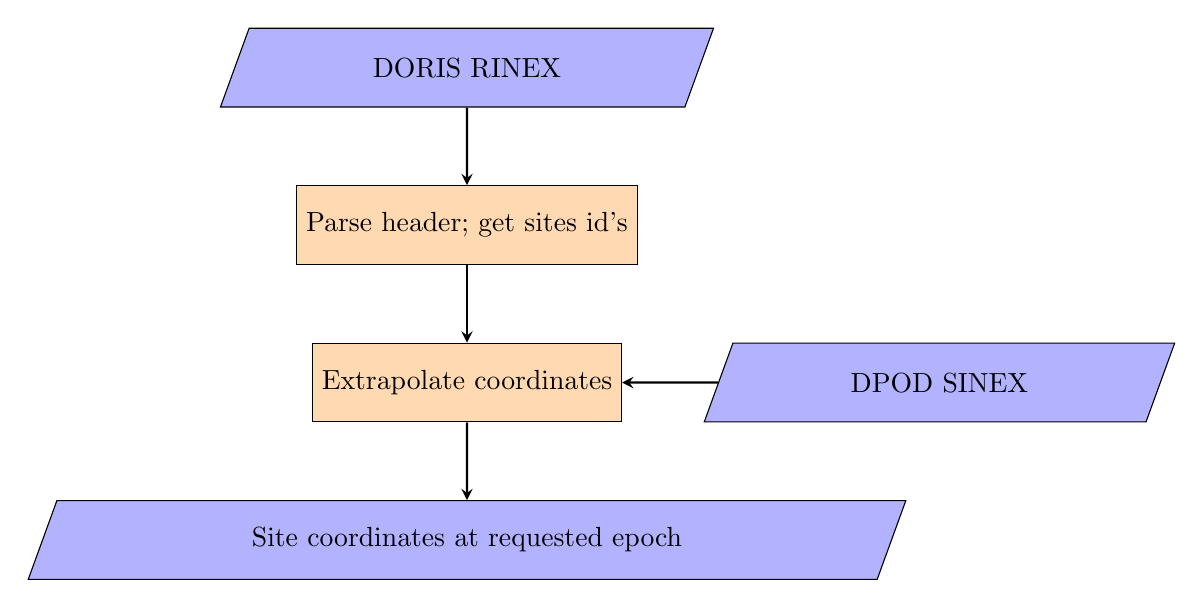
\begin{tikzpicture}[node distance=2cm]
\node (rnxin) [io] {DORIS RINEX};
\node (parsehdr) [process, below of=rnxin] {Parse header; get sites id's};
\node (xtrapolate) [process, below of=parsehdr] {Extrapolate coordinates};
\node (snxin) [io, right of=xtrapolate, xshift=4cm] {DPOD SINEX};
\node (out1) [io, below of=xtrapolate] {Site coordinates at requested epoch};
\draw [arrow] (rnxin) -- (parsehdr);
\draw [arrow] (parsehdr) -- (xtrapolate);
\draw [arrow] (snxin) -- (xtrapolate);
\draw [arrow] (xtrapolate) -- (out1);
\end{tikzpicture}

\section{DPOD}
For the analysis of DORIS observations, we need to have (at least approximate) 
site coordinates for the observed DORIS sites/beacons. Note that in DORIS RINEX 
v3 format \cite{DORISRNX3}, the RINEX files record all the observed sites at the 
file header, using the fields (among others):
\begin{itemize}
    \item 4-character station code,
    \item Station name (\textit{max 30characters long}) and 
    \item DOMES number
\end{itemize}

Example:
\begin{verbatim}
    51                                                      # OF STATIONS
D01  AMVB AMSTERDAM                     91401S005  3   0    STATION REFERENCE
D02  MAUB MARION ISLAND                 30313S005  3   0    STATION REFERENCE
...
D50  BADB BADARY                        12338S002  3   0    STATION REFERENCE 
D51  GRFB GREENBELT                     40451S178  3   0    STATION REFERENCE
\end{verbatim}

To match the sites with external sources (e.g. SINEX files), we will normally use 
the 4-character station code and/or the domes number.

In the meeting on the 15\textsuperscript{th} October 2021, it was suggested that instead of ITRF(2014, ...) 
we should better use the IDS published DPOD set of coordinates/veclocities (for better 
consistency). PDOP is a ``DORIS extension of the ITRF for Precise Orbit Determination'' 
estimated and delivered by the IDS Combination Center; details can be found on the 
\href{https://ids-doris.org/analysis-coordination/combination/dpod.html}{IDS DPOD webpage}.

Currently (October 2021) the latest PDOP realization is DPOD2014 \cite{Moreaux2019118} and 
the latest release is ``August 2020 - version \#5 - \textbf{dpod2014\_0}'' \cite{Moreaux2020};
the corresponding information files are published by 
\href{ftp://cddis.gsfc.nasa.gov/pub/doris/products/dpod/dpod2014/}{cddis} and
\href{ftp://doris.ensg.ign.fr/pub/doris/products/dpod/dpod2014/}{ign} in both 
SINEX and ascii/text format. Of the two, we are going to use the SINEX files (since 
they are more comprehensive, self-contained, capable of holding much more detailed information 
and widely used is Satellite Geodesy). 

Appropriate source code is written so as to be able to read and parse the DPOD SINEX 
file(s) and extrapolate site coordinates to a desired epoch. The sites we want to 
extrapolate coordinates for, are distinguished via their 4character id.

\section{Todo}
\subsection{Coordinate Std Deviations}
Also compute (extrapolated) coordinate stdandard deviations to go with the computed coordinate components.

\subsection{Ignored SINEX Sections}
The \textbf{dpod2014\_0} SINEX file contains a couple of blocks that (at this point) are 
not considered when parsing/extrapolating. These are (\cite{Moreaux2020}):
\begin{itemize}
    \item SOLUTION/DISCONTINUITY: origin (ex: earthquake, beacon change, antenna problem...) of
the position discontinuities
    \item SOLUTION/DATA\_REJECT: periods of time not included in the combination
    \item STATION/TO\_BE\_UPDATED: stations with non-negligible position change wrt DPOD2014v03
\end{itemize}

These are not crucial at this point but should be considered further on.

\section{Technicalities}

Main source code for the above is developed within the 
\begin{itemize}
    \item \href{https://github.com/xanthospap/libsinex}{sinex} and
    \item \href{https://github.com/xanthospap/doris}{doris}
\end{itemize}
repositories.

%The main function that does the work, is:
%\begin{lstlisting}
%#if __cplusplus >= 202002L
%template <typename T>
%    requires(T::is_of_sec_type && !std::is_same_v<T, dso::microseconds>)
%#else
%template <class T,
%          typename = std::enable_if_t<(T::is_of_sec_type) &&
%                                      (!std::is_same_v<T, dso::microseconds>)>>
%#endif
%int extrapolate_sinex_coordinates(
%            const char *snx_fn, char **site_ids, int num_sites,
%            const dso::datetime<T> &t) noexcept {
%    dso::datetime<dso::microseconds> t_micro =
%    t.template cast_to<dso::microseconds>();
%return extrapolate_sinex_coordinates(snx_fn, site_ids, num_sites, t_micro);
%}
%\end{lstlisting}

The following example (\href{https://github.com/xanthospap/doris/blob/main/test/test\_pdop\_crd.cc}{test\_pdop\_crd.cc}) 
extrapolates the coordinates of all the sites recorded in a DORIS RINEX file using a DPOD 
SINEX file. It is tested with the following SINEX files:
\begin{itemize}
    \item dpod2014\_053.snx
\end{itemize}

%\codelst{source/test_pdop_crd.cc}
\chapter{DORIS Ground Segment}
\label{ch:doris-ground-segment}

\tikzset{cross/.style={cross out, draw=red, minimum size=2*(#1-\pgflinewidth), inner sep=0pt, outer sep=0pt},
%default radius will be 1pt. 
cross/.default={1pt}}

\section{Geometry of Ground Antennae}
DORIS observations are referred to the electronic reference point (RP) of the antenna, 
the points where the DORIS observations  are  acquired.  As  that  electronic  point 
(\SI{2}{\GHz} center of phase for DORIS) is virtual and as for example it may change 
while using another type of antenna data referring to that electronic point are of no 
use for geophysical studies. So, observations must be referred to the conventional RP 
which is defined according to the geometry of the antenna. Therefore, one has also to 
account for the distance between the electronic RP and the conventional RP of the antenna (\cite{TOURAIN2016}). 
The ability to get accurate DORIS data relies for one part on the capability of providing 
accurate models to connect the  electronic RP (or electronic phase center) and the conventional 
RP, as well as, phase center variations (\gls{pcv}s) as a function of the elevation angle and azimuth.

The type of antenna is identified by the 4\textsubscript{th} character of the beacon 
mnemonic: letter ``A'' for the Alcatel type; letter ``B'' or letter ``C'' for the 
Starec B or C type.  That is, in the DORIS RINEX field ``STATION REFERENCE'', the 
last character of the second column (aka ``4-character station code''), defines the 
ground beacon antenna type; example:

\begin{adjustbox}{max width=\linewidth , fbox=0.5pt}
\begin{BVerbatim}[commandchars=\\\{\}]
    51                                                      # OF STATIONS       
D01  BEM\textcolor{red}{B} BELGRANO                      66018S002  3   0    STATION REFERENCE   
D02  ADH\textcolor{red}{C} TERRE ADELIE                  91501S005  3   0    STATION REFERENCE   
D03  SYQ\textcolor{red}{B} SYOWA                         66006S005  3   0    STATION REFERENCE   
D04  CRQ\textcolor{red}{C} CROZET                        91301S004  4   0    STATION REFERENCE   
D05  DIO\textcolor{red}{B} DIONYSOS                      12602S012  3   0    STATION REFERENCE
\end{BVerbatim}
\end{adjustbox}

\begin{table}[h!]
    \centering
    \begin{tabular}{|c | c | c | c | c|}
        \hline
        Zenith Distance & \multicolumn{2}{c}{ALCATEL (dBi)} & \multicolumn{2}{c|}{STAREC (dBi)} \\
                        & \SI{401.25}{\mega\hertz} & \SI{2036.25}{\mega\hertz} &  \SI{401.25}{\mega\hertz} & \SI{2036.25}{\mega\hertz}\\
        \hline
        \ang{0}&3.2&2.1&3.5&0 \\
        \ang{10}&3.5&2.6&3.6&0.4\\
        \ang{20}&4&2&3.7&0.5\\
        \ang{30}&4.4&4&3.8&1.5\\
        \ang{40}&4.6&4.4&3.7&3.2\\
        \ang{50}&4.2&4.6&3.2&3.9\\
        \ang{60}&2.7&2.7&2.5&4\\
        \ang{70}&0.6&-0.1&1&3.2\\
        \ang{80}&-2.7&-3.3&-1.3&0.2\\
        \ang{90}&-6&-7&-4.2&-5.6\\
        \hline
    \end{tabular}
    \caption{DORIS ground antennae gains, \cite{DORISGSM}.}
    \label{table:antenna-gains}
\end{table}

\subsection{Phase Center Offsets}

Depending on the antenna type, appropriate \gls{pco}s need to be applied to 
the observed quantities for the reduction of the observation vector to the Reference Point 
(from the respective ``virtual'' phase center) of the antenna. When a linear combination 
of the observed quantities is used, a respective \gls{pco} needs to be computed and 
applied. E.g., for the case of the Ionospheric-free linear combination, the respective 
\gls{pco} is:
\begin{equation}
    \vec{r}_{2GHz,iono-free} = \frac{\vec{r}_{400MHz,2GHz}}{\gamma - 1}
\end{equation}

where $\vec{r}_{2GHz,iono-free}$ is the vector from the \SI{2}{\GHz} phase
center to the iono-free phase center and $\vec{r}_{400MHz,2GHz}$ is
the vector from the \SI{400}{MHz} to the \SI{2}{\GHz} phase center.

\begin{table}[h!]
    \centering
    \begin{tabular}{|c|c|c|}
        \hline
        Antenna Type & ALCATEL & STAREC-B \& STAREC-C \\
        \hline
        $\Delta h$ in \si{\mm} for \SI{2}{\GHz} & \SI{510}{\mm} & \SI{487}{\mm}\\
        $\Delta h$ in \si{\mm} for \SI{400}{\MHz} & \SI{335}{\mm} & \SI{0}{\mm}\\
        \hline
    \end{tabular}
    \caption{DORIS ground antennae Phase Center Offsets, \cite{DORISGSM}.}
    \label{table:antenna-pco}
\end{table}

\subsection{DORIS ALCATEL Antenna}

\begin{figure}
\centering
\begin{tikzpicture}
    \draw (2,-2) -- (2,-7); %% left vertical
    \coordinate (LT) at (2,-2);
    \draw (5,-2) -- (5,-7); %% right vertical
    \coordinate (RT) at (5,-2);
    \coordinate (L2PC) at (3.5, -4.0);
    \coordinate (L1PC) at (3.5, -3.0);
    \coordinate (BRP) at (3.5, -7.0);
    \draw (LT) to[out=60, in=120] (RT); %% dome
    \draw (LT) to (RT); %% top horizontal (under dome)
    \draw (1,-7) -- (6,-7); %% reference plain
    \draw (1, -7) -- (1, -7.5); %% left minor vertical
    \draw (6, -7) -- (6, -7.5); %% right minor vertical
    \draw [line width=0.25mm] (0,-7.5) -- (9,-7.5); %% ground
    \draw [-stealth] (3.5,-7.5) --node[anchor=west]{local vertical} (3.5, -8.5); %% local vertical to ground
    \draw [dotted] (3.5, 0) -- (3.5, -7.5); %% local vertical from dome
    
    \draw (L1PC) circle (2pt) node[anchor=south west]{phase center \SI{2}{\GHz}}; %% 2GHz pc
    \draw (L1PC) node[cross=3pt, rotate=0] {}; %% 2GHz cross
    \draw [dotted] (L1PC) -- (9.5, -3.0); %% horizontal from 2GHz PC
    \path (9.5, -7.0) -- node[](hl1){h\textsubscript{2GHz} = \SI{510}{\mm}} (9.5, -3.0);
    \draw [<-] (9.5, -7.0)--(hl1); \draw [->] (hl1)--(9.5, -3.0);
    
    \draw (L2PC) circle (2pt) node[anchor=south west]{phase center \SI{400}{\MHz}}; %% 400 MHz pc
    \draw (L2PC) node[cross=3pt, rotate=0] {}; %% 400MHz cross
    \draw [dotted] (L2PC) -- (9, -4.0); %% horizontal from 400MHz PC
    \path (8, -7.0) -- node[](hl2){h\textsubscript{400MHz} = \SI{335}{\mm}} (8, -4.0);
    \draw [<-] (8, -7.0)--(hl2); \draw[->] (hl2)--(8, -4.0);
    
    \draw (BRP) circle (2pt) node[anchor=south west]{DORIS reference point}; %% reference point
    \draw (BRP) node[cross=3pt, rotate=0] {}; %% RP cross
    \draw [dotted] (BRP) -- (10, -7.0); %% horizontal from RP
    \draw (10, -7) node[anchor=north west]{DORIS reference plane};
    
    \node[rectangle, align=left] (rptext) at (-1,-3.5) {DORIS reference point \\ \(\begin{bmatrix} x_s y_s z_s \end{bmatrix}^{T} \) beacon \\position in earth reference \\frame};
    \draw [-stealth] (rptext) to ($(BRP)-(3pt,-3pt)$);
    \node[above,font=\large\bfseries] at (current bounding box.north) {ALCATEL DORIS Ground Antenna};
\end{tikzpicture}

\caption{Geometry of Alcatel DORIS Ground Antenna/Beacon}
\label{fig:alcatel-antenna}
\end{figure}


\subsection{DORIS STAREC Antenna}
STAREC antennae B and C are identical in terms of design and specification, the
difference is about the error budget in phase center position. For STAREC-C,
manufacturing process and error budget have been improved \cite{DORISGSM}.

According to \cite{TOURAIN2016}, in order to check the consistency of the theoretical 
characteristics of this type of antennae, a measurement campaign was performedby 
the CNES at the Compact Antenna Test Range (CATR). The CATR is a dedicated facility 
consisting ofan anechoic chamber equipped with several specific devices 
allowing significant measurement for satellite characterization.

As a result of the campaign, a phase law was established by averaging the estimated 
phase law values obtained during the CATR characterization. The resulting couple phase 
center position–phase law correction was provided to the  DORIS  users  through  a  
text  file  in  \gls{antex} (\cite{ANTEXv14}) format, available on the IDS website
\url{ftp://ftp.ids-doris.org/pub/ids/stations/doris_phase_law_antex_starec.txt}.

STAREC antennae B and C are identical in terms of design and specification, the
difference is about the error budget in phase center position. For STAREC C,
manufacturing process and error budget have been improved (\cite{DORISGSM}).

\begin{figure}
\centering
\tikzset{cross/.style={cross out, draw=red, minimum size=2*(#1-\pgflinewidth), inner sep=0pt, outer sep=0pt},
%default radius will be 1pt. 
cross/.default={1pt}}

\begin{tikzpicture}
    \coordinate (top) at (4,-1);
    \coordinate (tl) at (3.8, -1.3);
    \coordinate (tr) at (4.2, -1.3);
    \coordinate (blt) at (3.8, -3.0);
    \coordinate (brt) at (4.2, -3.0);
    \coordinate (blb) at (3.5, -3.3);
    \coordinate (brb) at (4.5, -3.3);
    \draw (top) to (tl);
    \draw (tl) to (blt);
    \draw (blt) to (blb);
    \draw (top) to (tr);
    \draw (tr) to (brt);
    \draw (brt) to (brb);
    \draw (blb) to (3.5, -9);
    \draw (brb) to (4.5, -9);
    \draw (3.5, -9) to (3.0, -9);
    \draw (3.0, -9) to (3.0, -9.3);
    \draw (4.5, -9) to (5.0, -9);
    \draw (5.0, -9) to (5.0, -9.3);
    \draw (3.0, -9.3) to (5.0, -9.3);

    \draw [dotted] (top) -- (4.0, -9.3); %% local vertical from top
    \draw [-stealth] (4.0, -9.3) -- node[anchor=west]{local vertical} (4.0, -10.3); %% local vertical arrow

    \coordinate (l1pc) at (4, -2.0);
    \draw (l1pc) circle (2pt) node[anchor=south west]{phase center \SI{2}{\GHz}}; %% 2GHz pc
    \draw (l1pc) node[cross=3pt, rotate=0] {}; %% 2GHz cross
    \draw (l1pc) to (10, -2.0);
    
    \coordinate (l2pc) at (4, -6.0);
    \draw [fill=black] (l2pc) circle (2pt) node[anchor=south west]{phase center \SI{400}{\MHz}}; %% 400MHz pc
    \draw (l2pc) node[cross=3pt, rotate=0] {}; %% 400MHz cross
    \draw ($(l2pc)-(1.0,0.0)$) -- node[below]{DORIS reference plane} (10, -6.0);
    \node (prt) at ($(l2pc)-(2.5,0.0)$) {Painted ring}; 
    \draw [-stealth] (prt) to ($(l2pc)-(0.2,0.0)$);

    \path ($(l1pc)+(5.5, 0.0)$) -- node[](h2g){h\textsubscript{2GHz} = \SI{487}{\mm}} ($(l2pc)+(5.5, 0.0)$);
    \draw [<-] ($(l1pc)+(5.5, 0.0)$) -- (h2g); 
    \draw [->] (h2g) -- ($(l2pc)+(5.5, 0.0)$);

    \node[rectangle, align=left] (rptext) at ($(l2pc)-(2.0,2.0)$) {DORIS reference point \\ \(\begin{bmatrix} x_s y_s z_s \end{bmatrix}^{T} \) beacon \\position in earth reference \\frame};
    \draw [-stealth] (rptext) to ($(l2pc)-(3.5pt,4.5pt)$);

    \node[above,font=\large\bfseries] at (current bounding box.north) {STAREC DORIS Ground Antenna};
\end{tikzpicture}

\caption{Geometry of Alcatel STAREC Ground Antenna/Beacon}
\label{fig:starec-antenna}
\end{figure}

\section{Phase Law}

\begin{tikzpicture}
\pgfplotstableread{tikz/phase_law.dat}{\table}
\begin{groupplot}[
  group style={
        group name= phase-law-plots,
        group size=1 by 2,
        xlabels at=edge bottom,
        xticklabels at=edge bottom,
        vertical sep=8pt,
    },
  %title={\texttt{patch type=quadratic spline}},
  xmin=0, xmax=90,
  ymin=-5, ymax=25,
  xtick distance = 5,
  ytick distance = 5,
  grid = both,
  minor tick num = 1,
  major grid style = {lightgray},
  minor grid style = {lightgray!25},
  width = \textwidth,
  height = 0.4\textwidth,
  xlabel = {Zenith angle ($^{\circ}$)},
]
\nextgroupplot[]
\addlegendimage{empty legend};
\addplot[blue, mark = *] table [x = {Zenith}, y = {Alcatel_1}] {\table};
\addlegendentry{\texttt{Alcatel Antenna}}[15 pt];
\coordinate (top) at (rel axis cs:0,1);% coordinate at top of the first plot

\nextgroupplot[]
\addlegendimage{empty legend};
\addplot[blue, mark = *] table [x = {Zenith}, y = {Starec_1}] {\table};
\addlegendentry{\texttt{Starec Antenna}}[15 pt];
\coordinate (bot) at (rel axis cs:0,0);% coordinate at bottom of the last plot

\end{groupplot}

\path (top-|current bounding box.west)-- node[anchor=south,rotate=90] 
  {Phase Correction for 2GHz ($mm$)} (bot-|current bounding box.west);

\path (top-|current bounding box.west) --
  node[anchor=south]{\textbf{DORIS Antennae Phase Law}} 
  (top-|current bounding box.east);
%\node (title) at ($(group c1r1.center)!0.5!(group c2r1.center)+(0,2cm)$) 
%  {DORIS Antenae Phase Law};
\end{tikzpicture}

%\begin{figure}
%\begin{subfigure}{0.45\textwidth}
%  \centering
%  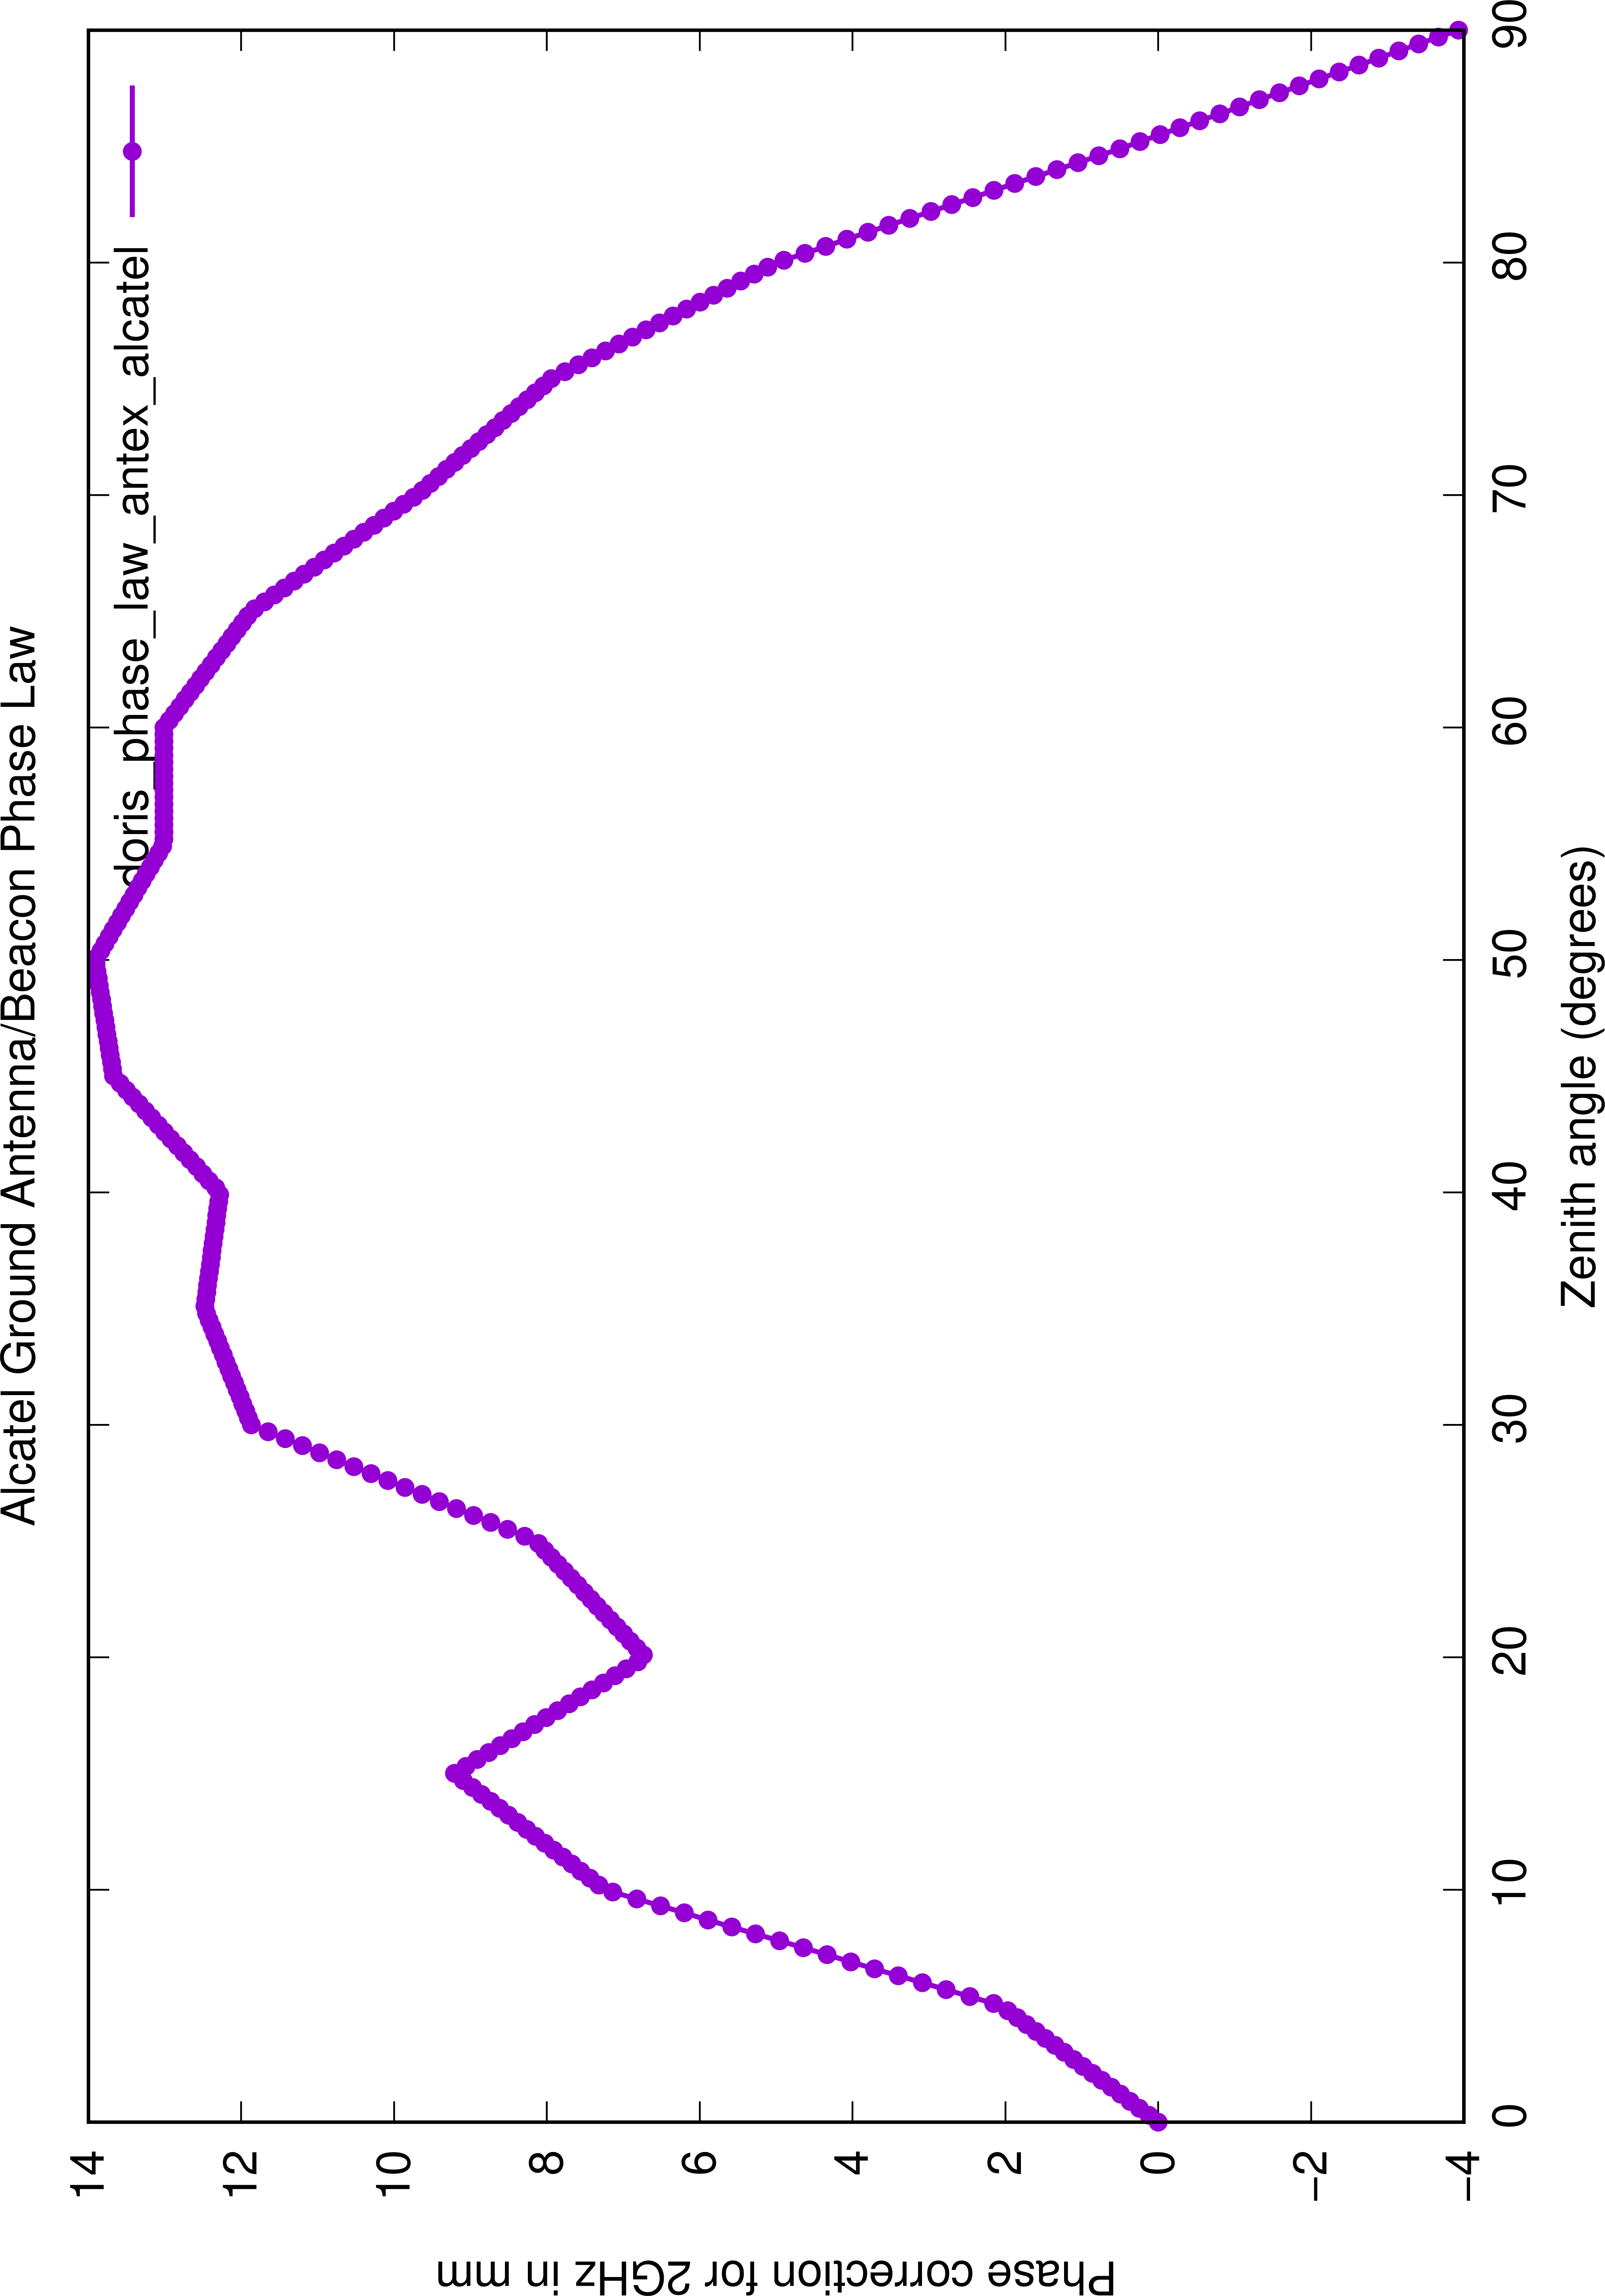
\includegraphics[width=.65\linewidth, angle=-90]{alcatel-phlaw}  
%  \caption{\scriptsize ALCATEL DORIS Ground Antenna Phase Law}
%  \label{fig:pcv-alcatel}
%\end{subfigure}
%\begin{subfigure}{0.45\textwidth}
%  \centering
%  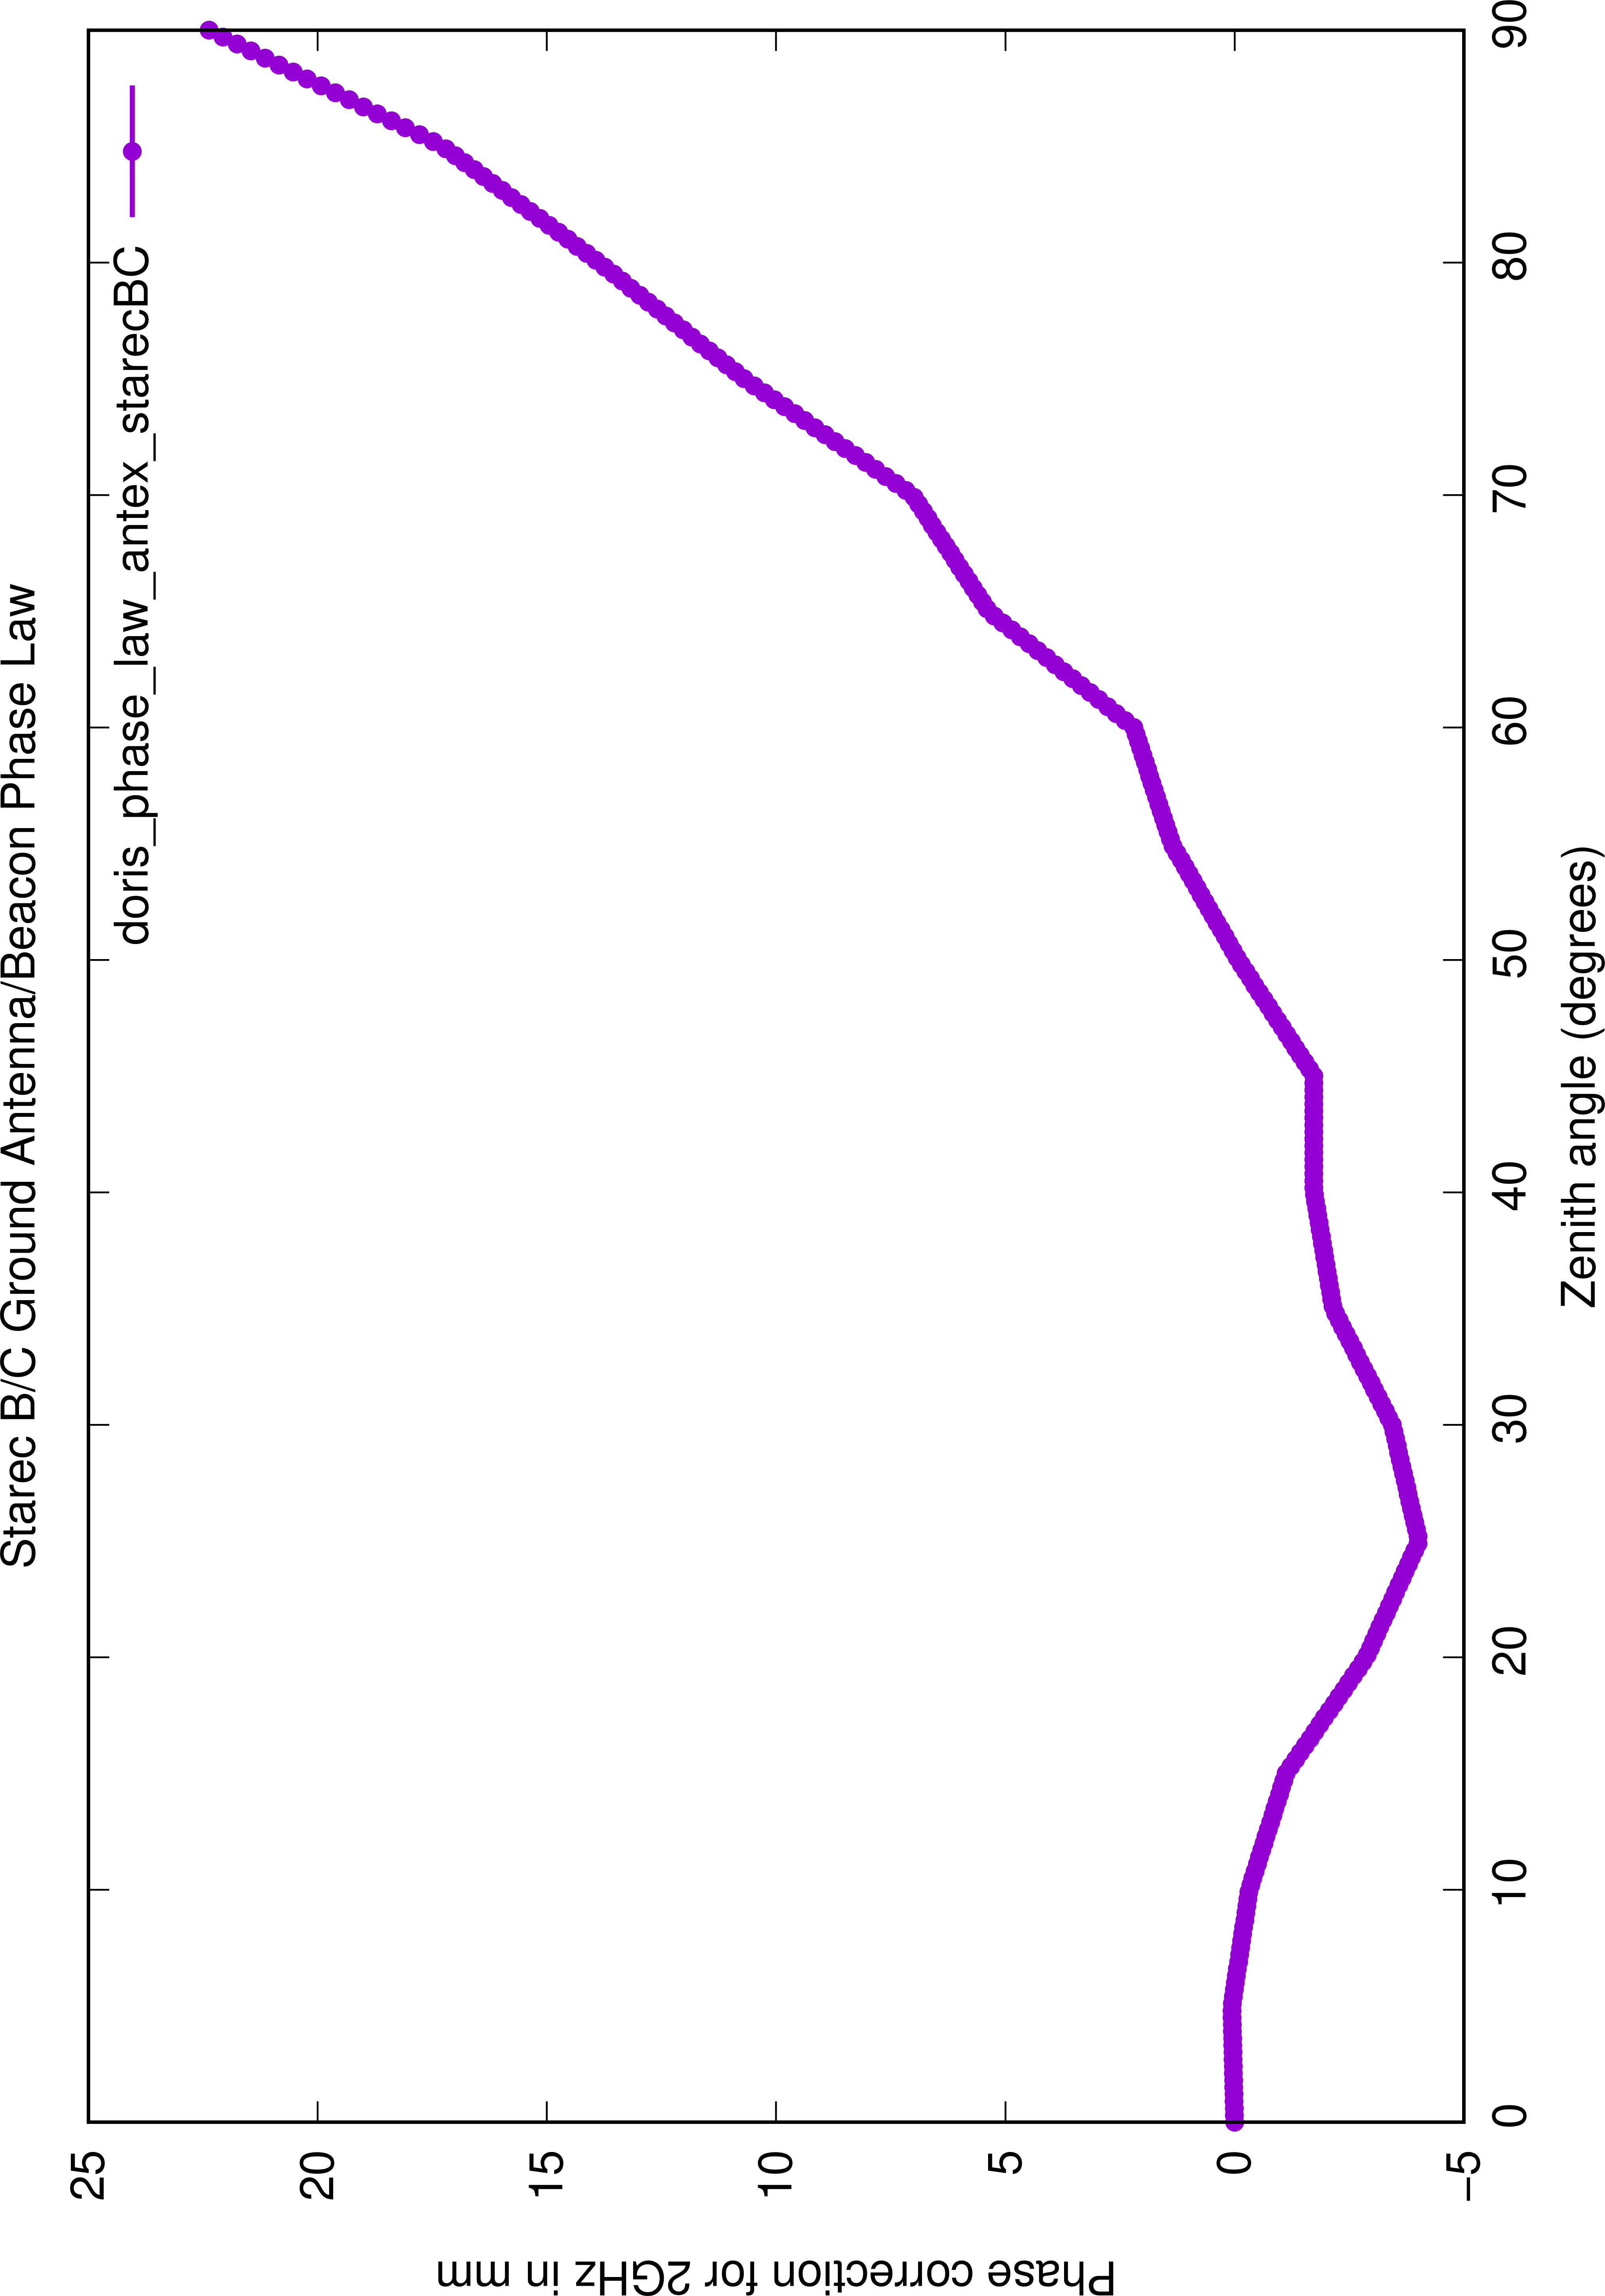
\includegraphics[width=.65\linewidth, angle=-90]{starecbc-phlaw}  
%  \caption{\scriptsize STAREC B/C DORIS Ground Antenna Phase Law}
%  \label{fig:pcv-starec}
%\end{subfigure}
%\caption{DORIS Ground Antenna Phase Law}
%\label{fig:ground-antenna-phase-law}
%\end{figure}


\bibliography{doris}

\glsaddall
\printglossary[type=\acronymtype,title=Acronyms]

\printindex

\end{document}